\label{sec:results_on_m2}
We tested StarNet on an SDSS image of the M2 globular cluster, a crowded starfield found in field 136 of camera column 2 in run 2583.
M2 was also imaged in the ACS Globular Cluster Survey~\cite{Sarajedini_2007}
using the Hubble Space telescope (HST),
which has approximately 20 times the angular resolution and 30 times the exposure of the Sloan telescope. The reported catalog from this Hubble survey serves as the ground truth for validating our results.

We consider the $100 \times 100$ subimage of M2 that \cite{Portillo_2017, Feder_2019} analyzed with PCAT.
This subimage is located approximately two arcseconds from the heavily saturated core of the cluster;
even in this subimage, the HST catalog contains over 1000 stars with F606W-band magnitudes less than 22.

Both StarNet and PCAT are able to model multiband images. We include two bands in our analysis, the SDSS $r$-band and $i$-band. 
The absorption ranges of the SDSS $r$-band and the Hubble F606W band are centered at roughly the same wavelength, but the absorption range of the Hubble F606W band is slightly broader. 

\subsection{Runtime} 
\label{sec:runtime}
The variational distribution factorizes into $2\times2$ tiles. 
The neural network inputs were $8\times8$ pixel padded tiles: 
$2\times 2$ tiles along with three surrounding pixels of padding (see Figure~\ref{fig:starnet_arch}). 
The SDSS estimates for the PSF and background were used in the first sleep phase. 
This phase ran for 200 epochs with 200 images per epoch with  
the Adam optimization routine~\cite{kingma2014adam}. 
On a single NVIDIA GeForce RTX 2080 Ti GPU, 
the initial sleep phase took 15.2 minutes.

Two additional wake-sleep cycles followed the first sleep phase. 
The subsequent sleep phases were shorter (10 epochs with 200 images each), and the wake phase employed SGD, with the gradient estimator \eqref{eq:mstep_grad}. In total, two further wake-sleep cycles took three minutes. 

After fitting the model and variational posterior, calculating the approximate posterior (that is, producing the distributional parameters of the variational approximation) for the $100 \times 100$ image of M2 took $29$ milliseconds. 
By comparison, the reported runtime of PCAT, which uses MCMC, is 30 minutes on the same $100 \times 100$ image~\cite{Feder_2019}.
In other words, after the initial fit, StarNet provided nearly a $10^5$-fold speed increase. 

The speed at inference time (which excludes training time) gives StarNet the scaling characteristics necessary for processing large astronomical surveys. 
A single SDSS image is $1489 \times 2048$ pixels. 
Based on the reported 30-minute runtime of PCAT for a $100\times100$ subimage, we project that
the runtime to process the full image would be $30\text{ min} \times 14 \times 20 = 8400$ minutes, or almost six days. 
The SDSS survey consists of nearly one million images. Scaling MCMC to the entire survey would be infeasible. 

In contrast, if we assume the PSF and background are homogeneous 
across the full SDSS image (which PCAT also assumes), we can 
fit StarNet using wake-sleep 
on a small $100 \times 100$ subimage
(while simultaneously obtaining estimates of the PSF and background),
a one time computational cost of 18.2 minutes. 
Producing a catalog with the full $1489 \times 2048$ image requires
$29\text{ msec} \times 14 \times 20 = 8.1$ seconds. In practice, 
inference can be made even faster by batching the image tiles to run in parallel on a GPU.

% An SDSS image is indexed by a run, camera column (camcol), and field.
% A run is one continuous scan of the telescope, usually corresponding to one night of data collection. 
% A run is broken down into fields; some runs have over 800 fields. 
% Each field contains six camera columns. 
% Thus, for a large-scale sky survey like SDSS which 
% consists of over 8000 runs for a total of nearly one million images, MCMC will be infeasible. 


\subsection{Inference}
\label{sec:results_on_m2_inference}
The cataloging accuracy of StarNet is compared with PCAT and DAOPHOT~\cite{stetson2987daophot}. 
DAOPHOT is an algorithmic routine for detecting stars in crowded starfields which does not use a generative model. 
This software convolves the observed image with a Gaussian kernel and scans for peaks above a given threshold. 
The DAOPHOT catalog of M2 was reported in \cite{An_2008_m2}. 


% Both DAOPHOT and the Hubble survey produce a single catalog -- that is, a set of estimated stellar locations and fluxes -- with
% error bars nominally representing marginal uncertainties.
% In the context of probabilistic cataloging (StarNet and PCAT), the posterior 
% defines a distribution over catalogs.
% Each sample from the (approximate) posterior returns a catalog, and each 
% sampled catalog may have different cardinally. 

To evaluate the three methods, the HST catalog was used as ground truth. 
We filtered the HST catalog to stars with magnitudes smaller than 22.5 in the Hubble F606W band because stars with lower apparent brightness cannot be detected in SDSS images. 


Estimated catalogs are evaluated on three metrics: the true positive rate (TPR), the positive predicted value (PPV), and the F1 score. The TPR is the proportion of stars in the HST catalog matched with a star in the estimated catalog;
the PPV is the proportion of stars in the estimated catalog matched with a star in the HST catalog. The F1 score summarizes the two metrics as the harmonic average between the PPV and the TPR.

Like \cite{Portillo_2017, Feder_2019}, a ``match" between an estimated star and an HST star is defined as follows: (1) the estimated location and the HST location are within 0.5 pixels, and (2) the estimated SDSS $r$-band flux and the HST F606W band flux are within half a magnitude. 

In probabilistic cataloging (PCAT and StarNet), the posterior defines a distribution over catalogs. 
To evaluate the TPR, PPV, and F1 score for PCAT, 300 catalogs were sampled using MCMC; the metrics were computed for each sampled catalog and averaged. 
For StarNet, the TPR, PPV, and F1 score were computed for the catalog corresponding to the mode of the variational distribution (henceforth, the StarNet catalog). 

% \jeff{A lot of sentences that have ``we'' as the subject can be rewritten in way that doesn't mention us (without switching to passive voice, which often doesn't sound good). It makes the writing easier to understand because typically ``we'' are not really central to the idea we're trying to convey. 
% So you might say thing like ``Our method performed better than PCAT in terms of TPR and PPV'' rather than all four of the follow sentences: ``We compute the the TPR and PPV for our method. We compared it to PCAT. We found that our method performed better than PCAT. Note that we used the MAP estimate to compute TPR.''
% }

Fitting StarNet using wake-sleep (StarNet-WS) resulted in a catalog that outperforms DAOPHOT and PCAT in terms of its F1 score (Table~\ref{tab:summary_stats}). 
Fitting StarNet without the wake phase
and using only the default SDSS background and PSF (StarNet-S) produced a catalog with a TPR similar to that of StarNet-WS but with a smaller PPV.
PCAT estimated the most stars of all methods, and it therefore had a large TPR but a small PPV. 
On the other hand, DAOPHOT estimated less than half the number of stars when compared to the other methods. It therefore had a large PPV but a small TPR. 
The StarNet-WS catalog had the same PPV as DAOPHOT while having nearly the same TPR as PCAT. 

% \begin{table}[!tb]
% \centering
% \caption{Performance metrics on M2.
% For probabilistic methods (StarNet and PCAT)
% the ``\#stars" column refers to the mean number of stars under the (approximate) posterior, while the right-most column displays the 5-th and 95-th percentiles under the posterior. }
% \label{tab:summary_stats}
% \begin{tabular}{l|ccc|cc}
% \toprule
%      Method &   TPR &   PPV &  F1 score &  \#stars & (q-5\%, q-95\%)\\
% \midrule
%     DAOPHOT &  0.20 &  0.63 &      0.30 &     295 & -- \\
%        PCAT &  0.56 &  0.40 &      0.47 &    1672 & (1664, 1680)\\
%  Sleep-only &  0.51 &  0.47 &      0.49 &    1292 & (1260, 1324)\\
%  Wake-sleep &  0.51 &  0.60 &      0.55 &     1014 & (987, 1041)\\
%      %Hubble &  1.00 &  1.00 &      1.00 &     1114 & -- %\\
% \bottomrule
% \end{tabular}
% \end{table}

\begin{table}[!tb]
\centering
\caption{Performance metrics on M2.
For probabilistic methods (StarNet and PCAT)
the ``\#stars" columns provide the mean along with the 5th and 95th percentiles
for the number of stars under the (approximate) posterior,
The number of stars in the Hubble catalog is 1114. }
\label{tab:summary_stats}
\begin{tabular}{l|ccc|cc}
\toprule
& & & & \multicolumn{2}{c}{\#Stars} \\
     Method &   TPR &   PPV &  F1 score &  mean & (q-5\%, q-95\%)\\
\midrule
    DAOPHOT &  0.20 &  0.65 &      0.31 &     357 & -- \\
       PCAT &  0.55 &  0.37 &      0.44 &    1672 & (1664, 1680)\\
 StarNet (our) &  0.53 &  0.48 &      \textbf{0.50} &    1462 & (1430, 1497)\\
\bottomrule
\end{tabular}
\end{table}


The improvement of StarNet-WS in PPV was most pronounced for dim stars (Figure~\ref{fig:summary_stats}). The TPR for StarNet-WS was uniformly better than DAOPHOT for stars of all magnitudes. 
Of all methods, the StarNet-WS catalog best approximated the Hubble flux distribution (Figure~\ref{fig:luminosity_fun_m2}). 
PCAT overestimated the number of dim stars with magnitudes less than 21. 
In contrast, DAOPHOT failed to find dim stars; its flux distribution assigned zero probability to stars with magnitudes greater than $21$.

\begin{figure}[ht]
    \centering
    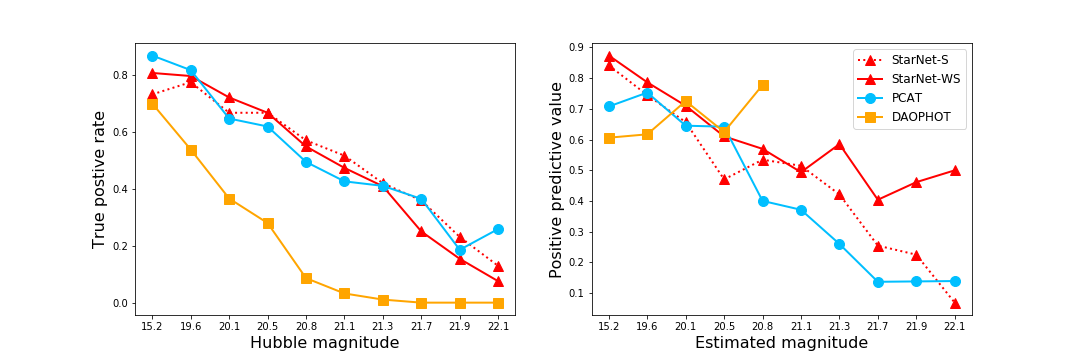
\includegraphics[width=0.99\textwidth]{figures/summary_statistics_m2.png}
    \caption{True positive rate and positive predicted value of various cataloging
    procedures on M2, plotted against magnitude.
    Smaller magnitudes correspond to brighter stars. 
    X-axis ticks correspond to Hubble magnitude deciles, so
    each bin contains roughly the same number of stars.  }
    \label{fig:summary_stats}
\end{figure}

\begin{figure}[ht]
    \centering
    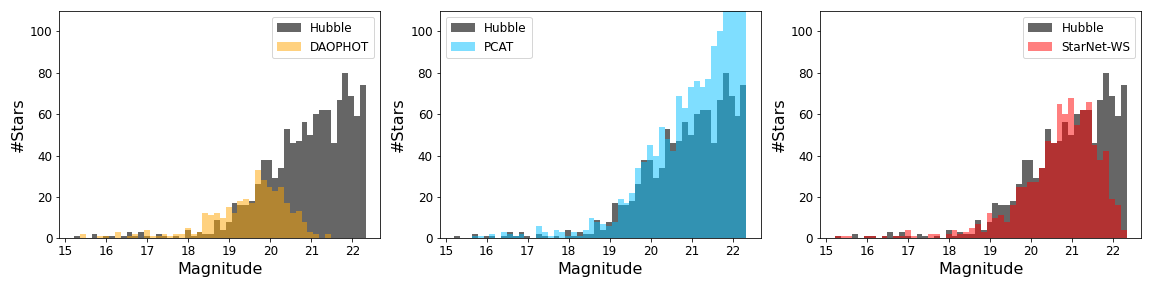
\includegraphics[width=0.99\textwidth]{figures/luminosity_fun.png}
    \caption{Source magnitude histograms for the $r$-band of M2. 
    The magnitude distribution of the Hubble catalog in grey. 
    Magnitude distributions for the DAOPHOT, PCAT, and StarNet-WS catalogs overlaid.
    For PCAT, the distribution comes from a single catalog sampled by MCMC. }
    \label{fig:luminosity_fun_m2}
\end{figure}

Figure~\ref{fig:example_subimages} shows the StarNet-WS catalog alongside PCAT, DAOPHOT, and Hubble catalogs. 

\begin{figure}[ht]
    \centering
    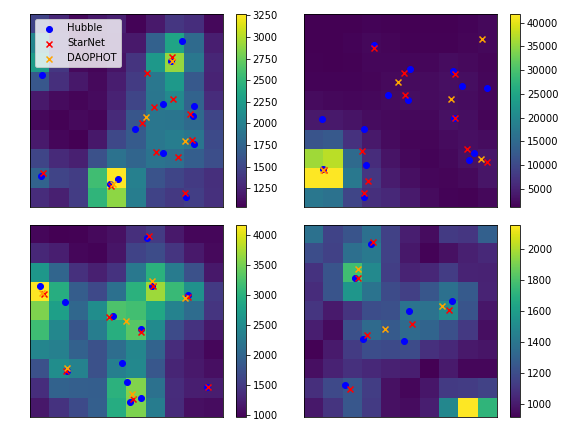
\includegraphics[width=0.49\textwidth]{figures/example_subimages_ws.png}
    \rulesep
    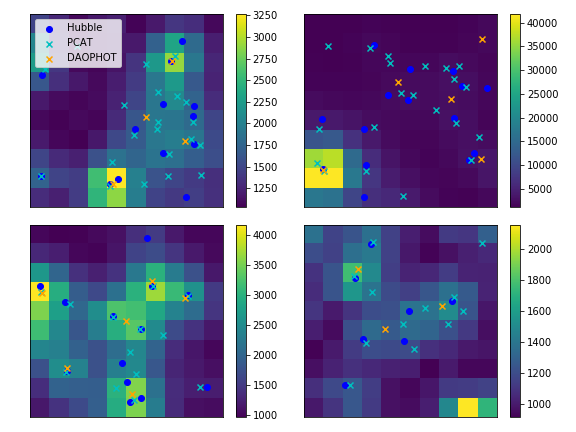
\includegraphics[width=0.49\textwidth]{figures/example_subimages_pcat.png}
    \caption{Estimated catalogs on four 10$\times$10 subimages from
    M2. Blue dots are stars from the HST catalog used as ground truth. 
    Starnet-WS, PCAT, and DAOPHOT estimated stars are shown as
    red, cyan, and orange crosses, respectively. }
    \label{fig:example_subimages}
\end{figure}

\begin{figure}[ht]
    \centering
    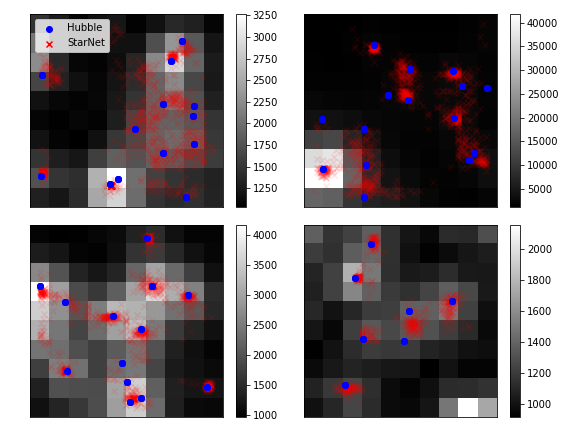
\includegraphics[width=0.49\textwidth]{figures/example_subimages_samples_ws.png}
    \rulesep
    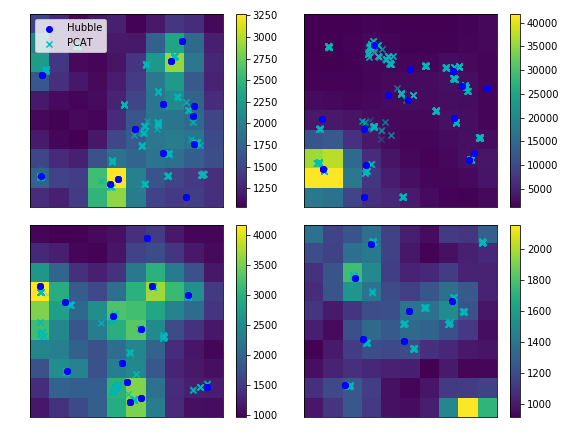
\includegraphics[width=0.49\textwidth]{figures/example_subimages_samples_pcat.png}
    \caption{Four 10$\times$10 subimages from
    M2. Blue dots are stars from the HST catalog used as ground truth. (Left) Posterior samples from StarNet-WS and (right) posterior samples from the MCMC chain of PCAT. }
    \label{fig:example_subimages_sampled}
\end{figure}

StarNet-WS returns a well-defined distribution over the set of all catalogs
and is thus able to capture uncertainties in catalog construction. 
Samples from the StarNet-WS variational distribution are compared with samples from PCAT in Figure~\ref{fig:example_subimages_sampled}. 
To examine the uncertainty calibration of StarNet-WS, we evaluated the approximate posterior 
conditional on the true number of stars in the Hubble catalog. 
Then, each star in the StarNet-WS catalog was matched with exactly one Hubble star by finding the permutation of Hubble stars that had the largest log-likelihood under our variational distribution $q_\eta$. 
For each star, we computed the z-score $(y - \hat y) / \hat \sigma$, where $y$ is the Hubble log-flux or 
logit-location; $\hat y$ and $\hat\sigma$ are the mean and the standard deviation, respectively, of the Gaussian variational distribution for the log-flux or logit-location.
If the uncertainties were perfectly calibrated, the distribution of the z-scores would be a standard Gaussian. 
The tails of the empirical z-score distribution are close to a standard Gaussian with some discrepancy in the tails, suggesting the uncertainties are only slightly under-estimated (Figure~\ref{fig:z-score_calibration}). 

\begin{figure}[ht]
    \centering
    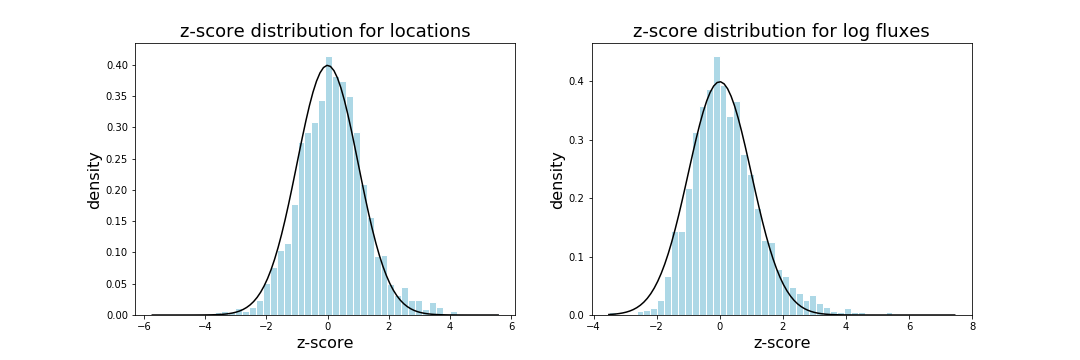
\includegraphics[width=0.99\textwidth]{figures/z-score_calibration.png}
    \caption{The empirical distribution of z-scores for logit-locations or log-fluxes under the StarNet-WS variational posterior. 
}
    \label{fig:z-score_calibration}
\end{figure}


% Figure~\ref{fig:cmd_m2} displays the estimated color-magnitude diagrams. While the Hubble F606W-band corresponds roughly to the SDSS $r$-band, there is no such correspondence for the SDSS $i$-band. Thus, using the Hubble locations, we estimated the $i$-band fluxes using maximum likelihood: letting $x^{(i)}$ be the SDSS image in the $i$-band, $N_H$ the number of stars in the Hubble catalog and $\ell_H$ their locations, solve
% \begin{align}
%   f^{(i)}_H = \argmax_{f\in\mathbb{R}^{N_H}} \log p(x^{(i)} | N_H, \ell_H, f)
%   \label{eq:optim_iband_flux},
% \end{align}
% where the log likelihood is given by the generative model from Section~\ref{sec:gen_model}.
% The estimated $i$-band fluxes and the reported Hubble F606W-band fluxes $f_H^{(r)}$ define the ``true" colors, $2.5\log(f_H^{(i)}/f_H^{(r)})$. 
% In the color magnitude diagram, DAOPHOT did not capture the full spectrum of colors; of all three methods, PCAT best captured the color spectrum. All three methods however, were able to capture the arm thing (TODO there is a name for this ... main sequence turnoff?) that branches off at low magnitudes. 

% \begin{figure}[ht]
%     \centering
%     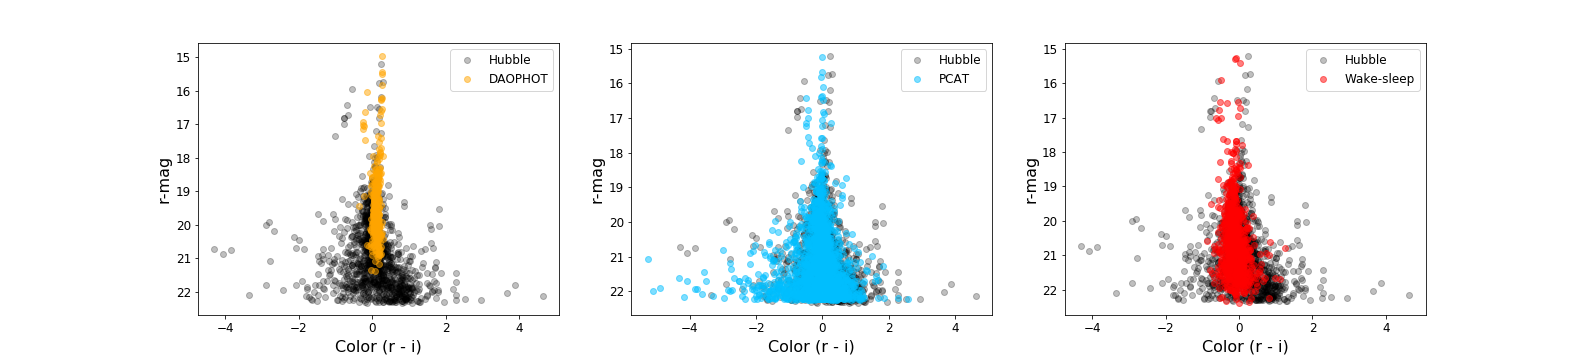
\includegraphics[width=0.99\textwidth]{figures/cmd.png}
%     \caption{Color magnitude diagrams on M2. }
%     \label{fig:cmd_m2}
% \end{figure}


Finally, we evaluate the quality of the wake phase estimates for the PSF and background. Let $z_h$ denote the Hubble catalog, and given some model parameters $\phi$, let
\begin{align}
    \mathcal{L}^{Hubble}(\phi) := 
    - \log \; p_\phi(x^{(r)} | z_h)
    \label{eq:hubble_neg_loglik}
\end{align}
be the negative log-likelihood of the SDSS $r$-band image conditional on the Hubble catalog (recall that the Hubble absorption range most closely resembles the SDSS $r$-band). The log-likelihood of model parameters estimated by the wake phase is nearly four times larger than the log-likelihood of parameters estimated by SDSS~(Table~\ref{tab:chi-square-stats1}). 
The largest improvement in log-likelihood came from the wake estimated background, suggesting that the SDSS background was a poor fit on this starfield. 

% \begin{table}[ht]
% \centering
% \caption{The negative log-likelihood \eqref{eq:hubble_neg_loglik} for various model estimates. PHOTO provides the SDSS estimates of background and PSF for every data release. 
% We compare the PHOTO estimates with StarNet estimates of the PSF and background obtained using wake-sleep. }
% \label{tab:chi-square-stats1}
% \begin{tabular}{lr}
% \toprule
%           Model Estimate & Neg. Loglik \\
% \midrule
%                      PHOTO background, PHOTO PSF&    1.88e+06 \\
%               PHOTO background, StarNet PSF &    1.86e+06 \\
%       StarNet background, PHOTO PSF &    4.94e+05 \\
%  StarNet background, StarNet PSF &    4.80e+05 \\
% \bottomrule
% \end{tabular}
% \end{table}

\begin{table}[ht]
\centering
\caption{The negative log-likelihood \eqref{eq:hubble_neg_loglik} for various model estimates. PHOTO provides the SDSS estimates of background and PSF for every data release. 
We compare the PHOTO estimates with StarNet estimates of the PSF and background obtained using wake-sleep. }
\label{tab:chi-square-stats1}
\begin{tabular}{lrr}
\toprule
\multicolumn{2}{c}{Model estimate} & Neg.Loglik \\
\cmidrule(lr){1-2} background & PSF &  \\
\midrule
PHOTO & PHOTO & 1.88e+06\\
PHOTO & StarNet & 1.86e+06 \\
StarNet & PHOTO & 4.94e+05\\
StarNet & StarNet & 4.80e+05 \\
\bottomrule
\end{tabular}
\end{table}

% Figure~\ref{fig:loglik_table} displays the log-likelihood under the default SDSS estimates of the PSF and background compared with the estimates found using wake-sleep. 
% The wake-sleep estimates improved the log-likelihood.
% We also compared against the ``Hubble estimate" of the background and PSF, obtained by minimizing $- \log p_\phi(x | N_{H}, \ell_{H}, f_{H})$ for $\phi$ directly. 

% The results suggest that the primary source of model misfit is the background. A significant increase in log-likelihood occurred by switching from the SDSS background to the Hubble-estimated background. 
% But even using the Hubble-estimated background, switching from the SDSS PSF to our wake-sleep PSF improves the log-likelihood. 

% \begin{figure}[ht]
%     \centering
%     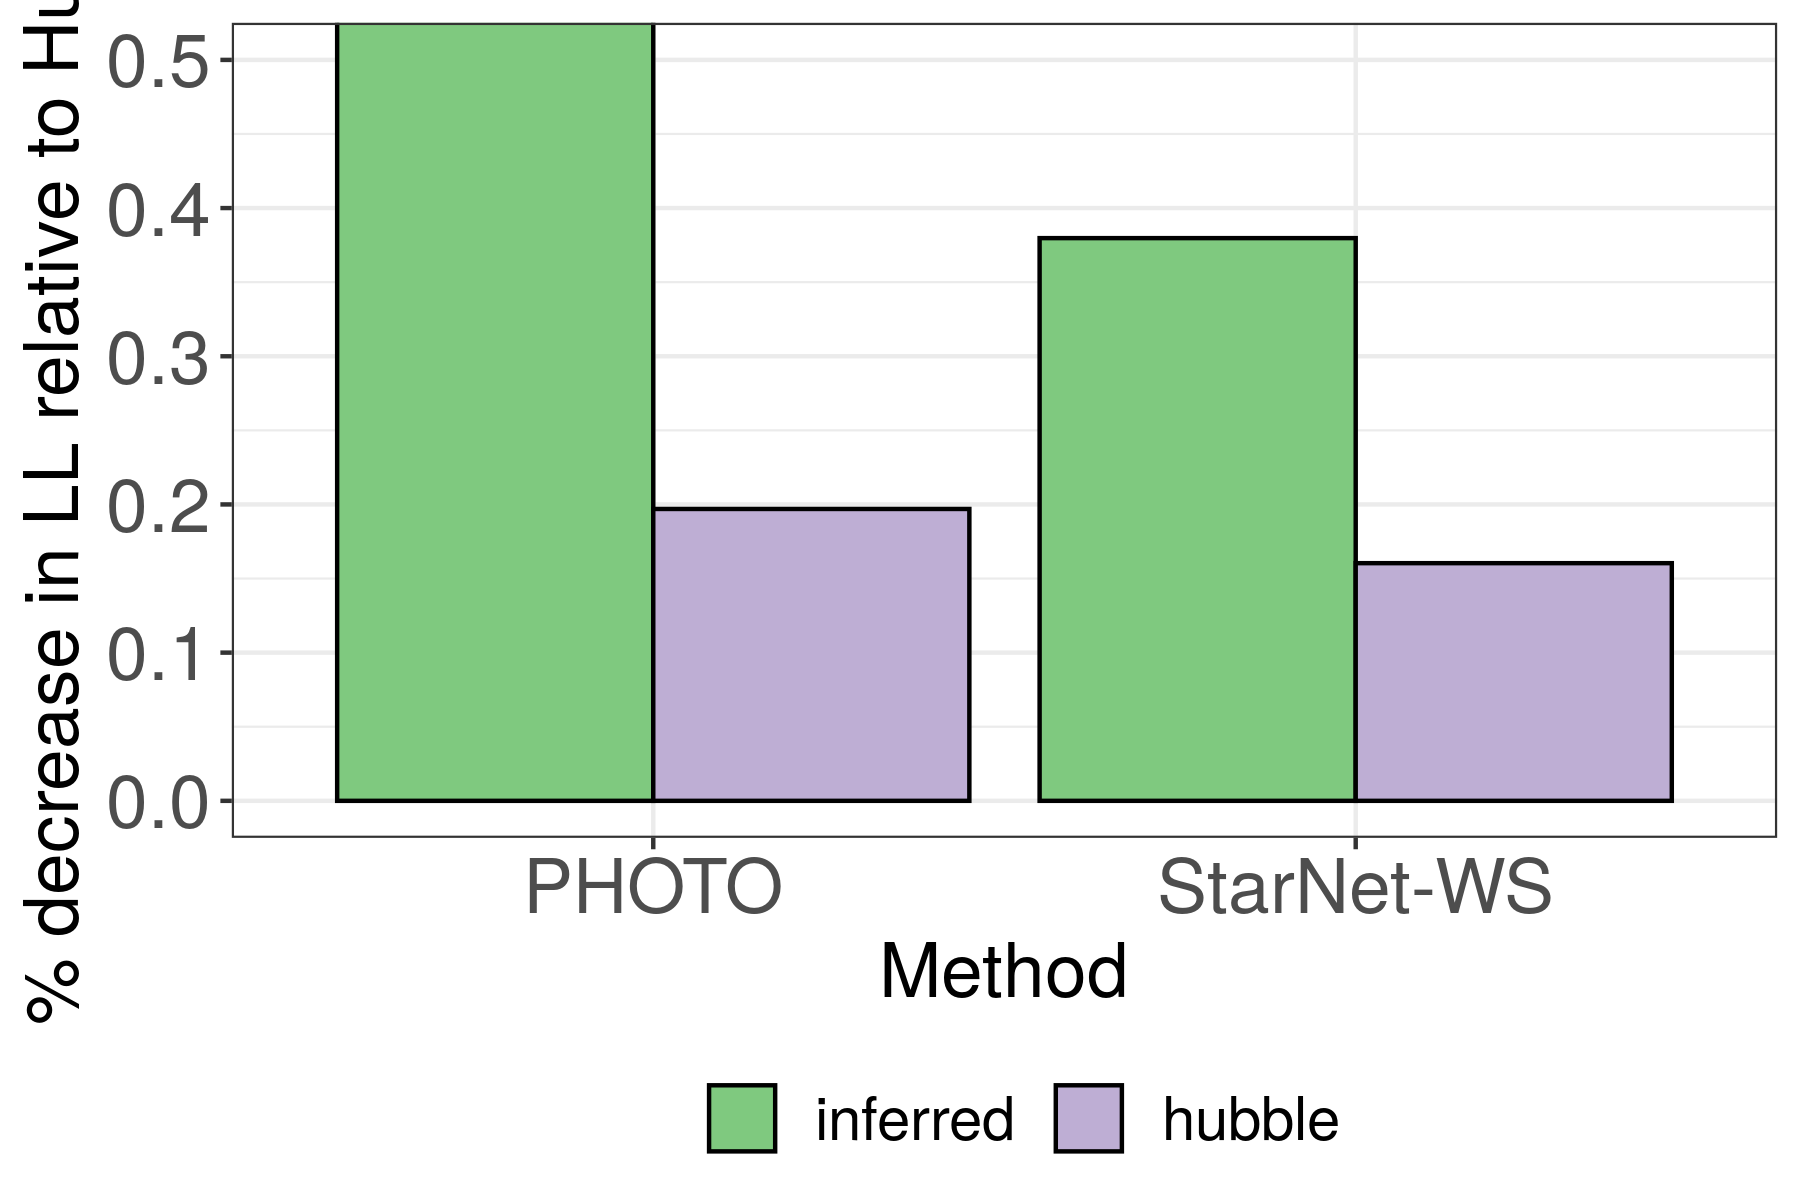
\includegraphics[width=0.6\textwidth]{figures/loglik_table.png}
%     \caption{Percent decrease in log-likelihood relative to the Hubble estimate of the PSF and background. 
%     For each method, we evaluate the log-likelihood where the both PSF 
%     and background are estimated (green); 
%     we also show results where only the PSF is estimated (purple). 
%     }
%     \label{fig:loglik_table}
% \end{figure}

% \input{tables/chi_sq_stats.txt}
% \caption{
% Negative log-likelihood for SDSS, wake-sleep, and Hubble estimated model parameters. In the right column, we fix the background to the Hubble estimate, and examine negative log-likelihood as the PSF varies.}

% The StarNet-based PSF did not differ from the SDSS PSF significantly. The greatest change was in the $r$-band PSF, where the SDSS PSF was most different from the Hubble-estimated PSF. 

% \begin{figure}[ht]
%     \centering
%     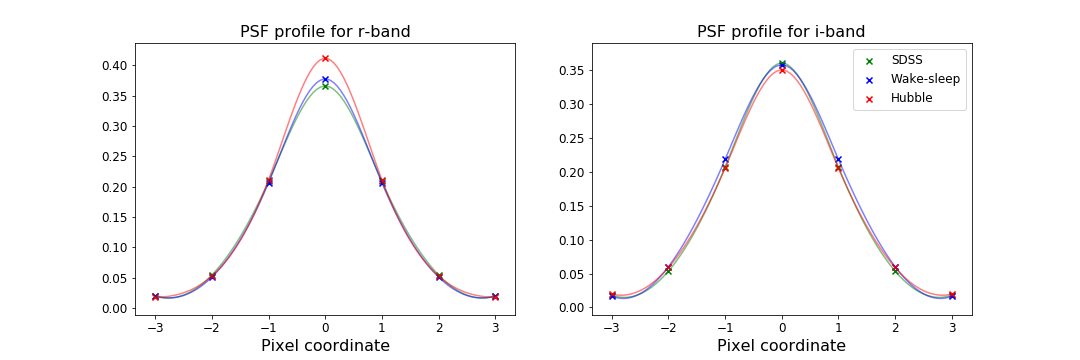
\includegraphics[width=0.99\textwidth]{figures/psf_profiles.png}
%     \caption{Estimated versus true PSF profiles on M2. The Hubble PSF was
%     obtained by optimizing the likelihood conditioned on locations and fluxes
%     from the Hubble catalog. TODO: this image is not that informative, I think I'll remove this. }
%     \label{fig:psf_profiles}
% \end{figure}


% \multicolumn{1}{p{5cm}}{\raggedleft Neg. loglik \\ (with Hubble back.)}
% \caption{
% Chi-squared statistics for SDSS, wake-sleep, and Hubble estimated model parameters.
% The chi-squared statistic is defined as
% $\sum_{bij}\frac{([\text{obs.image}]_{bij} - [\text{recon.image}]_{bij})^2}{[\text{recon.image}]_{bij}}$.
% In the middle column, ``model parameters" refer to both background and PSF.
% In the right column, we fix the background to the Hubble estimate, and examine
% chi-squared statistics as the PSF varies.}

